\documentclass[12pt]{beamer}

\usepackage{tikz}
\usepackage{graphicx}
\usepackage[T1]{fontenc}
\usepackage{amsmath}
\usepackage{multicol}
\usepackage{booktabs, braket} % For formal tables
\usepackage{cleveref}
\usepackage{graphicx}
\usepackage{blkarray}
\usetikzlibrary{graphs, graphs.standard}

\DeclareMathOperator{\E}{\textrm{E}}		     % expected value
\DeclareMathOperator{\pr}{\mathrm{P}}		     % probability 
\DeclareMathOperator{\cov}{t_{cov}}	             % cover time

\DeclareMathOperator{\X}{\mathbb{X}}		     % expected value
\DeclareMathOperator{\tr}{\text{tr}}		     % trace
\DeclareMathOperator{\Ap}{$A$ ^\prime} 		     % A'
\DeclareMathOperator{\bp}{$b$ ^\prime} 		     % b'
\DeclareMathOperator{\Xb}{\mathcal{X}}		     % big X

\newcommand\coolover[2]{\mathrlap{\smash{\overbrace{\phantom{%
    \begin{matrix} #2 \end{matrix}}}^{\mbox{$#1$}}}}#2}

\newcommand\coolunder[2]{\mathrlap{\smash{\underbrace{\phantom{%
    \begin{matrix} #2 \end{matrix}}}_{\mbox{$#1$}}}}#2}

\newcommand\coolleftbrace[2]{%
#1\left\{\vphantom{\begin{matrix} #2 \end{matrix}}\right.}

\newcommand\coolrightbrace[2]{%
\left.\vphantom{\begin{matrix} #1 \end{matrix}}\right\}#2}

\title{Semidefinite Programming and Quantum Algorithms}
\author{Michael Czekanski \& R. Teal Witter}
\institute{Middlebury College}
\date{December 3, 2019}

\newcommand{\todo}[1]{{\color{red}{[{\bf TODO:} #1]}}}

\begin{document}
\graphicspath{{./../figures/}}

\frame{\titlepage}

\begin{frame}{Overview}
\setcounter{tocdepth}{1}
\tableofcontents
\end{frame}

\section{Introduction}
\begin{frame}{Motivation}
As quantum computers someday soon maybe might become a reality...
\newline
\newline
What are the problems that quantum computers 
can solve more efficiently
than classical computers? \#QuantumSpeedUp

\end{frame}

\begin{frame}{Houston, we have a problem:}
Given Boolean function $f$...
\newline
\newline
What is the optimal quantum query complexity?
\newline
\newline
What is a query optimal quantum algorithm?
\end{frame}

\section{Background}
\begin{frame}{Query Complexity}
Given bitstring $x$ and function $f$,
how many bits of $x$ to determine $f(x)$ in the worst case?
\only<2-3>
{
\begin{align}
 f: x_1 \wedge (x_2 \vee \bar{x_2}) \vee x_3 \nonumber
\end{align}
}
\only<3>
{
\begin{align}
x &\rightarrow f(x) \nonumber \\
000 &\rightarrow 0 \nonumber \\
010 &\rightarrow 0 \nonumber \\
011 &\rightarrow 1 \nonumber
\end{align}
}
\only<4-5>
{
\begin{align}
 f: x_1 \vee x_2 \vee x_3 \nonumber
\end{align}
}
\only<5>
{
\begin{align}
x &\rightarrow f(x) \nonumber \\
000 &\rightarrow 0 \nonumber \\
010 &\rightarrow 1 \nonumber \\
011 &\rightarrow 1 \nonumber
\end{align}
}
\end{frame}

\begin{frame}{Span Program}
Given $x$ and $f$, is $f(x)$ true?
$$\iff$$
Given input vectors $I(x)$ and target vector $\tau$,
do the input vectors span to the target vector?
\newline
\newline
\only<2->
{
For OR, $I(x) = x$ and $\tau = 1$.
}
\newline
\newline
\only<3>
{
I(000) = {0,0,0} does not span to $\tau$
:(
}
\only<4>
{
I(010) = {0,1,0} does span to $\tau$
:)
}
\end{frame}

\section{Our Work}


\begin{frame}{Our Approach, Generally} 
\centering
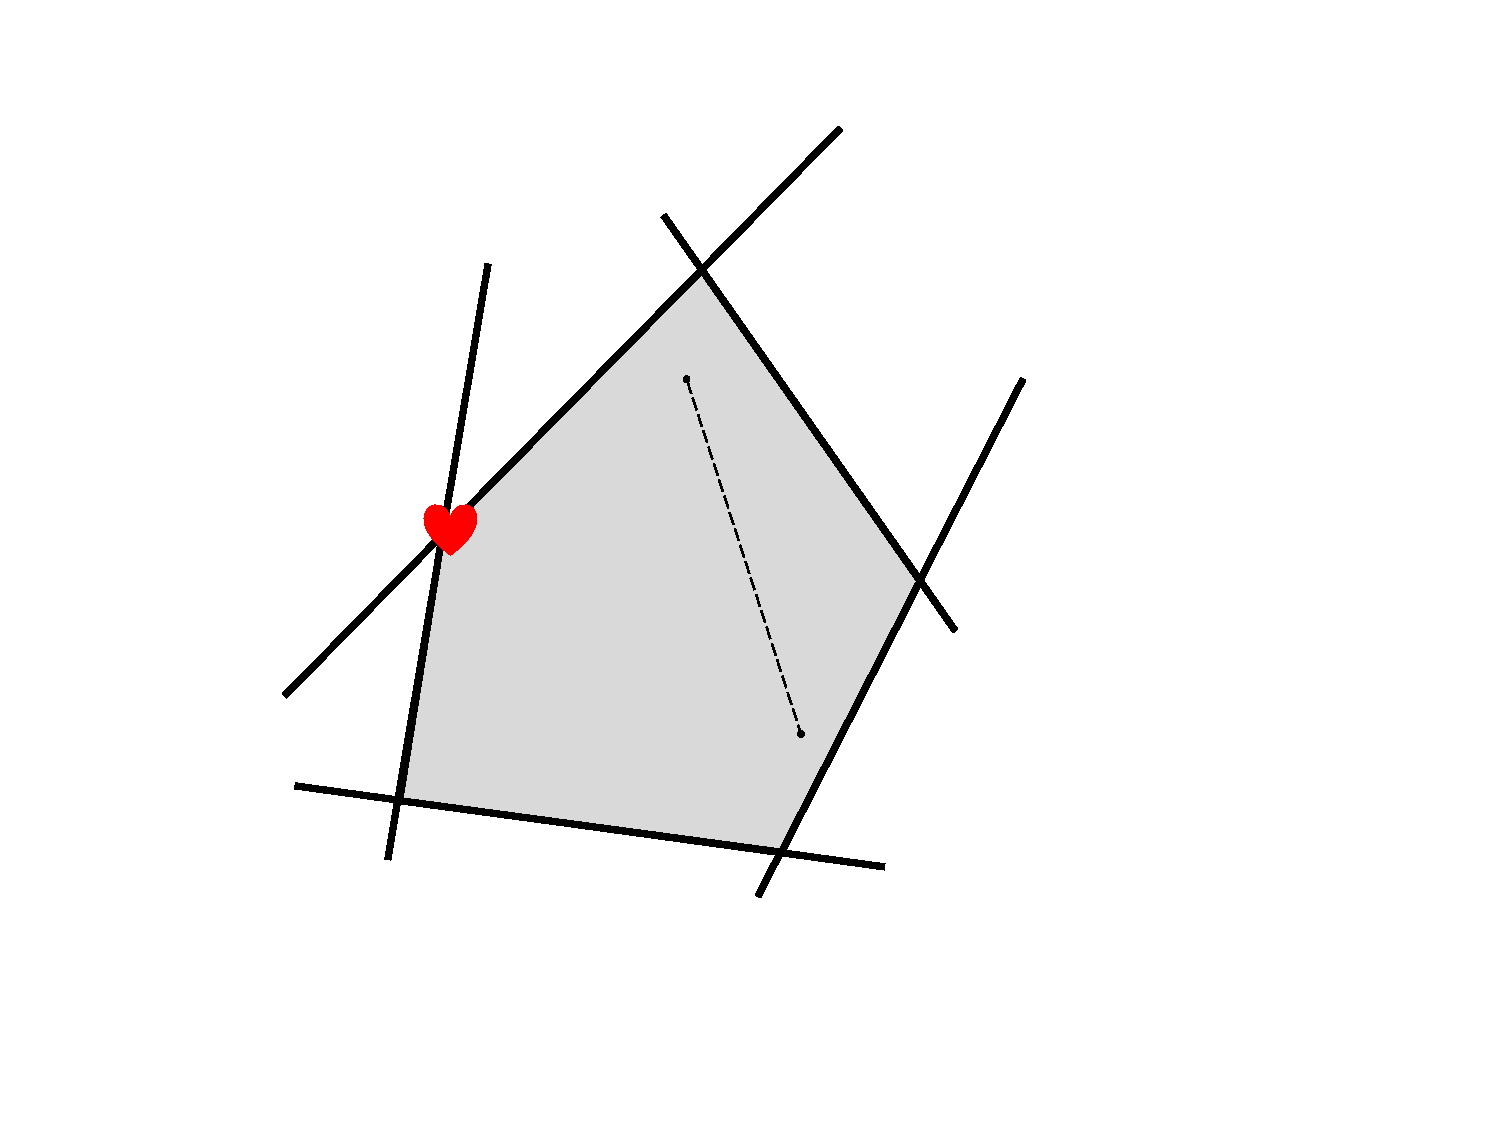
\includegraphics[scale=.5]{convex_optimization.pdf}
\end{frame}

\begin{frame}{Our Approach, Specifically \cite{reichardt2009span}}
\begin{align} \label{eq:reichardtObj} 
    f_{\text{bound}} = \min_{\X} \left( \max_{y \in D} \sum_{j \in [n]}
    \bra{y,j}\X\ket{y,j}  \right) \nonumber
\end{align}
Subject to:
\begin{align}\label{Eq:reichardtSemi}
    \X \succcurlyeq 0 \nonumber
\end{align}
\begin{align}\label{Eq:reichardtOffDiag}
    \forall (y,z) \in F \sum_{j \in [n]: y_j \ne z_j} 
    \bra{y,j} \X \ket{z, j} = 1 \nonumber
\end{align}
\end{frame}

\begin{frame}{What $\X$ Looks Like (2-bit OR)}
    \begin{align}
\X = \begin{blockarray}{ccccc}
\qquad & 00 & 01 & 10 & 11 \\
\begin{block}{c[cccc]}
  00 & X_{(00,00)} & X_{(00,01)} & X_{(00,10)} & X_{(00,11)}\\
  01 & X_{(01,00)} & X_{(01,01)} & X_{(01,10)} & X_{(01,11)}\\
  10 & X_{(10,00)} & X_{(10,01)} & X_{(10,10)} & X_{(10,11)}\\
  11 & X_{(11,00)} & X_{(11,01)} & X_{(11,10)} & X_{(11,11)}\\
\end{block}
\end{blockarray} \nonumber 
\end{align}
\end{frame}

\begin{frame}{What $\X$ Looks Like (2-bit OR)}
    \begin{align}
    \X = \left[ \begin{array}{cc|cc|cc|cc}
    0.7 & 0 & 0 & 0 & 1 & 0 & 0.5 & 0\\
    0 & 0.7 & 0 & 1 & 0 & 0 & 0 & 0.5\\
    \hline
    0 & 0 & 0 & 0 & 0 & 0 & 0 & 0\\
    0 & 1 & 0 & \sqrt{2} & 0 & 0 & 0 & 0.7\\
    \hline
    1 & 0 & 0 & 0 & \sqrt{2} & 0 & 0.7 & 0\\
    0 & 0 & 0 & 0 & 0 & 0 & 0 & 0\\
    \hline
    0.5 & 0 & 0 & 0 & 0.7 & 0 & 0.6 & 0\\
    0 & 0.5 & 0 & 0.7 & 0 & 0 & 0 & 0.6\\
    \end{array}
\right] \nonumber
\end{align}
\end{frame}

\begin{frame}{What $\X$ Looks Like (2-bit OR)}
    We want to minimize the maximum (over inputs $y$) of:
    \begin{align}
         \sum_{j \in [n]}
    \bra{y,j}\X\ket{y,j}   \nonumber
    \end{align}
    \begin{align}
    \X = \left[ \begin{array}{cc|cc|cc|cc}
    \color{blue}0.7 & 0 & 0 & 0 & 1 & 0 & 0.5 & 0\\
    0 & \color{blue}0.7 & 0 & 1 & 0 & 0 & 0 & 0.5\\
    \hline
    0 & 0 & \color{orange}0 & 0 & 0 & 0 & 0 & 0\\
    0 & 1 & 0 & \color{orange}\sqrt{2} & 0 & 0 & 0 & 0.7\\
    \hline
    1 & 0 & 0 & 0 & \color{purple}\sqrt{2} & 0 & 0.7 & 0\\
    0 & 0 & 0 & 0 & 0 & \color{purple}0 & 0 & 0\\
    \hline
    0.5 & 0 & 0 & 0 & 0.7 & 0 & \color{cyan}0.6 & 0\\
    0 & 0.5 & 0 & 0.7 & 0 & 0 & 0 & \color{cyan}0.6\\
    \end{array}
\right] \nonumber
\end{align}
\end{frame}

\begin{frame}{What $\X$ Looks Like (2-bit OR)}
    For $y,z$ such that $f(y) \neq f(z)$:
    
    \begin{align}
         \sum_{j \in [n]: y_j \ne z_j} 
    \bra{y,j} \X \ket{z, j} = 1 \nonumber
    \end{align}
    \begin{align}
    \X = \begin{array}{cc|cc|cc|cc}
    0.7 & 0 & \color{blue}0 & 0 & \color{orange}1 & 0 & \color{cyan}0.5 & 0\\
    0 & 0.7 & 0 & \color{blue}1 & 0 & \color{orange}0 & 0 & \color{cyan}0.5\\
    \hline
    \color{blue}0 & 0 & 0 & 0 & 0 & 0 & 0 & 0\\
    0 & \color{blue}1 & 0 & \sqrt{2} & 0 & 0 & 0 & 0.7\\
    \hline
    \color{orange}1 & 0 & 0 & 0 & \sqrt{2} & 0 & 0.7 & 0\\
    0 & \color{orange}0 & 0 & 0 & 0 & 0 & 0 & 0\\
    \hline
    \color{cyan}0.5 & 0 & 0 & 0 & 0.7 & 0 & 0.6 & 0\\
    0 & \color{cyan}0.5 & 0 & 0.7 & 0 & 0 & 0 & 0.6\\
    \end{array} \nonumber
\end{align}
\end{frame}


\subsection{How We Get Our $\X$}
\begin{frame}{We use ADM \cite{adm}}
\centering
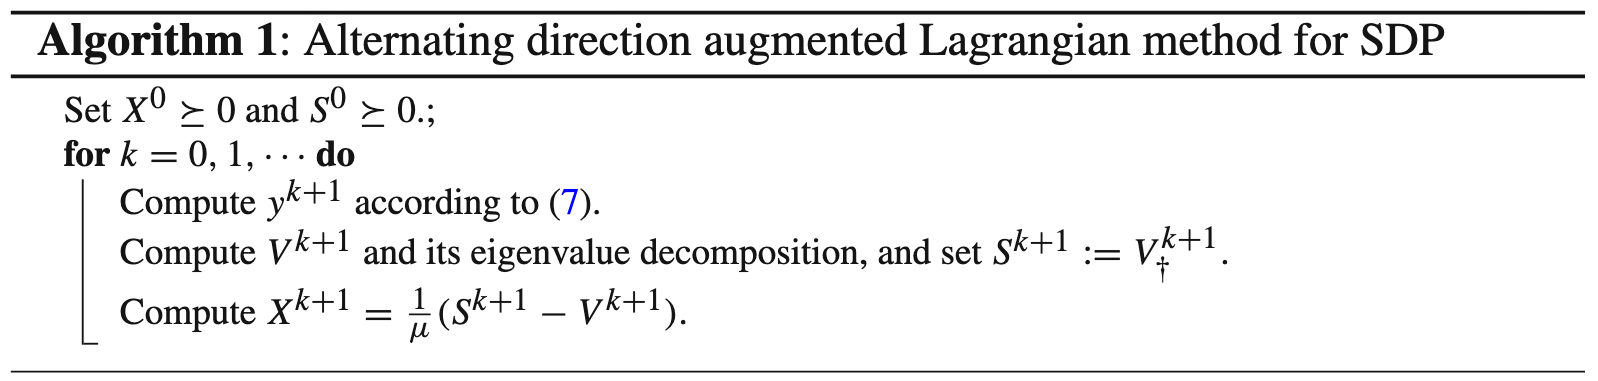
\includegraphics[scale=.15]{figures/adm_algorithm}
\bigskip
\begin{itemize}
    \item "Easy" to implement
    \item Exploits sparsity
\end{itemize}
\end{frame}

\begin{frame}{Numerical Results: Very Accurate :)}
\centering
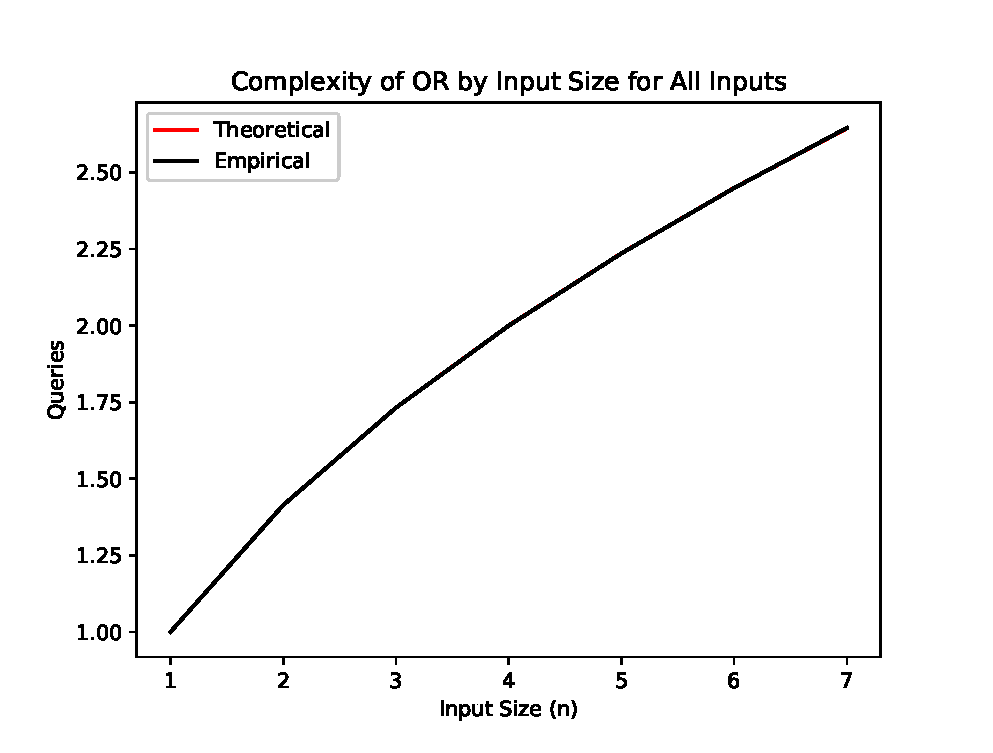
\includegraphics[scale=.5]{or_all_complexity.eps}
\end{frame}

\begin{frame}{Run Time Results: Too Many Inputs :(}
\centering
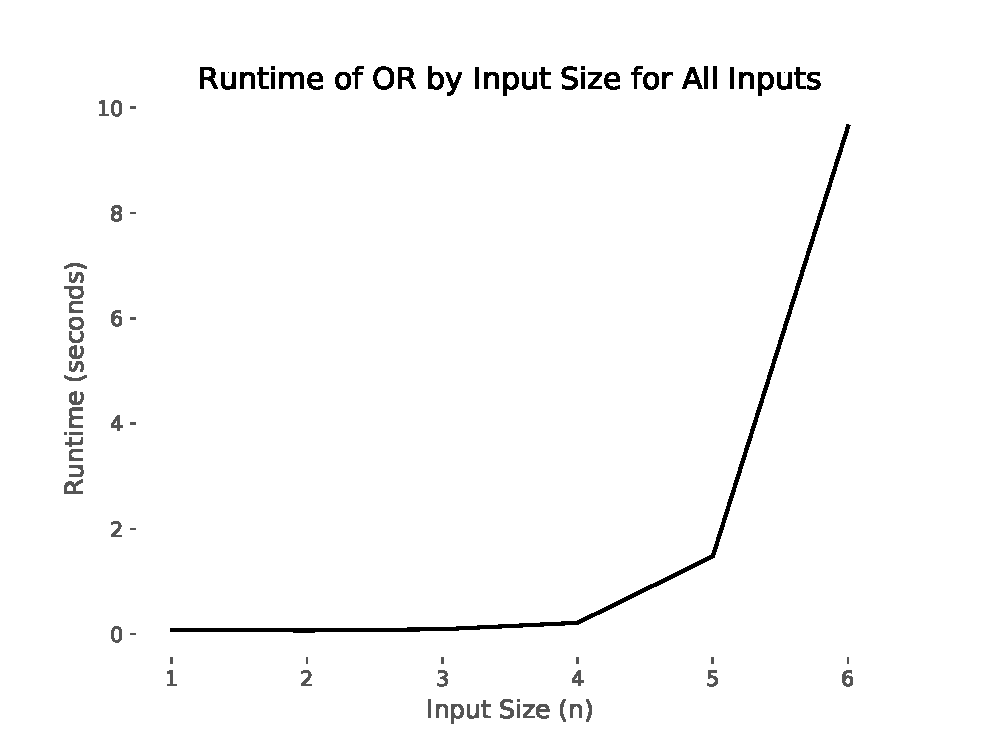
\includegraphics[scale=.5]{or_all_runtime.eps}
\end{frame}

\begin{frame}{In Conclusion...}
    \begin{itemize}
        \item Our algorithm rocks
        \item Except on large inputs
    \end{itemize}
\end{frame}

\section{Future Work}
\begin{frame}{Future Work}
\begin{itemize}
    \item Expand our algorithm beyond binary outputs
    \item Utilize a more efficient solver
    \item Memory efficiency of span programs
\end{itemize}
\end{frame}

\begin{frame}{Thank you!}
\bibliographystyle{abbrv}
\bibliography{main}
\end{frame}

\end{document}